\documentclass[11pt,a4paper]{article}
\usepackage[margin=2.5cm]{geometry}
\usepackage{amsmath,amssymb}
\usepackage{booktabs}
\usepackage{enumitem}
\usepackage{xcolor}
\usepackage{tikz}
\usetikzlibrary{patterns}
\usepackage[colorlinks=true,linkcolor=blue!50!black]{hyperref}

\definecolor{boxbg}{HTML}{EEF3F8}
\definecolor{zoneF}{HTML}{CFE3F7}
\definecolor{haloF}{HTML}{FFD9B3}
\definecolor{ink}{HTML}{43505C}
\definecolor{agent}{HTML}{C0392B}
\newcommand{\idea}[1]{\par\smallskip\noindent\colorbox{boxbg}{\parbox{\dimexpr\linewidth-2\fboxsep}{\textbf{Key idea.} #1}}\par\smallskip}

\title{Reading guide\\[2pt]\large The halo, the boundary protocol of the section-based controller}
\author{Companion to \texttt{Chapters/4.Implementation.tex} (\texttt{eq:halo})}
\date{}

\begin{document}
\maketitle

\noindent This guide explains how a section-based controller sees across
the edge of its own zone. It adds no new model. Everything here points back
to \texttt{eq:halo} in the Method chapter and to the row ``zone-local state,
boundary protocol'' of \texttt{tab:information}. The design is logged as
\texttt{[A6]} in \texttt{thesis-progress/temp/GAPS.md}.

\tableofcontents

%----------------------------------------------------------------
\section{The problem the halo solves}

A section-based controller cuts the warehouse into zones $Y_1,\dots,Y_p$
and runs one network per zone, all with the same weights. If each network
saw only its own zone, an agent standing right at a zone edge would be
blind to everything one step across it. It could walk into an agent it had
no way of seeing, and its crowding count $\delta_i(t)$ would stop at the
edge, so the same number would mean something different here than under
the other two controllers.

The halo gives each zone a narrow, read-only view across its edge.

%----------------------------------------------------------------
\section{The definition}

\[
  H_q = \{\, v \notin Y_q : d_G(w,v) \le d_{\mathrm{obs}} \text{ for some } w \in Y_q \,\}.
\]

\noindent In words, the halo of zone $Y_q$ is every vertex \emph{outside}
the zone that is within $d_{\mathrm{obs}}$ hops of some vertex
\emph{inside} it. It is a band of the neighbouring zones, exactly as deep as
an agent's field of view.

\idea{The halo is the boundary protocol. In \texttt{tab:information},
``zone-local state, boundary protocol'' means the zone itself plus its halo,
nothing more.}

%----------------------------------------------------------------
\section{How it works, step by step}

\begin{enumerate}[label=\arabic*.,leftmargin=*]
  \item \textbf{The network runs on the zone plus the halo.} Zone $Y_q$'s
        network takes $Y_q \cup H_q$ as its graph.
  \item \textbf{The halo is read-only.} Halo vertices carry only their
        role (storage, delivery, endpoint, transit) and whether an agent is
        standing there. They have no action heads and add nothing to the
        loss. The zone sees across its edge but never decides there.
  \item \textbf{A zone owns the agents inside it.} It chooses an action
        only for agents with $\ell_i(t) \in Y_q$. An agent standing in the
        halo is visible, but it belongs to the neighbouring zone.
  \item \textbf{Handover.} When an agent steps into the next zone, that
        zone takes ownership on the same timestep. Every zone uses the same
        weights, so only the agent's context changes, not the policy that
        decides for it.
  \item \textbf{Conflicts across the edge.} Two zones can each propose a
        move onto the same boundary vertex. The shared conflict-resolution
        operator removes that clash, the same way it removes any other.
        That operator is part of the environment, not part of any
        controller's window, so using it at a boundary does not let a zone
        see more.
\end{enumerate}

%----------------------------------------------------------------
\section{A small example}

Take a graph like the small one of \texttt{fig:controllers-example}, three rows and
four columns. Let zone $Y_1$ be the left two columns and let
$d_{\mathrm{obs}} = 1$. The halo $H_1$ is then the third column, one hop
past the edge. The fourth column is two hops away and is not in the halo.

\begin{center}
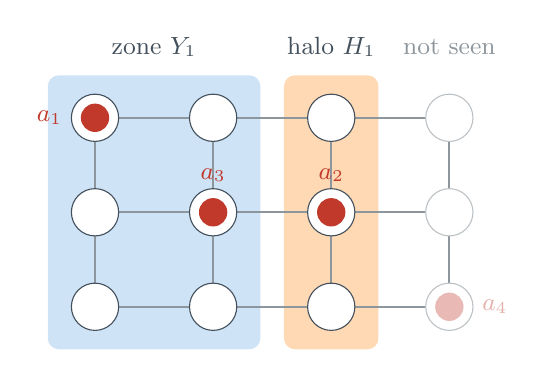
\begin{tikzpicture}[x=1.5cm,y=1.2cm,
    v/.style={circle,draw=ink,fill=white,minimum size=6mm,inner sep=0pt},
    ag/.style={circle,fill=agent,minimum size=3.6mm,inner sep=0pt}]
  % zone and halo backgrounds
  \fill[zoneF,rounded corners=4pt] (-0.4,-0.45) rectangle (1.4,2.45);
  \fill[haloF,rounded corners=4pt] (1.6,-0.45) rectangle (2.4,2.45);
  \node[font=\small,text=ink] at (0.5,2.75) {zone $Y_1$};
  \node[font=\small,text=ink] at (2,2.75) {halo $H_1$};
  \node[font=\small,text=ink!60] at (3,2.75) {not seen};
  % edges
  \foreach \r in {0,1,2} \foreach \c in {0,1,2} \draw[ink!60,line width=0.8pt] (\c,\r) -- (\c+1,\r);
  \foreach \r in {0,1} \foreach \c in {0,1,2,3} \draw[ink!60,line width=0.8pt] (\c,\r) -- (\c,\r+1);
  % vertices
  \foreach \r in {0,1,2} \foreach \c in {0,1,2} \node[v] at (\c,\r) {};
  \foreach \r in {0,1,2} \node[v,draw=ink!35] at (3,\r) {};
  % agents
  \node[ag] at (0,2) {}; \node[font=\small,text=agent,left=2pt] at (-0.15,2) {$a_1$};
  \node[ag] at (1,1) {}; \node[font=\small,text=agent,above=4pt] at (1,1.1) {$a_3$};
  \node[ag] at (2,1) {}; \node[font=\small,text=agent,above=4pt] at (2,1.1) {$a_2$};
  \node[ag,opacity=0.35] at (3,0) {}; \node[font=\small,text=agent!40,right=2pt] at (3.15,0) {$a_4$};
\end{tikzpicture}
\end{center}

\begin{itemize}[leftmargin=*]
  \item $Y_1$'s network decides for $a_1$ and $a_3$, the agents inside
        the zone.
  \item It sees that the halo vertex next to $a_3$ is occupied, by $a_2$.
        So $a_3$'s crowding count includes $a_2$, exactly as it would under
        the decentralised or centralised controller. But $Y_1$ does not
        choose $a_2$'s action. $a_2$'s own zone does.
  \item It does not see $a_4$, two hops past the edge.
  \item If $a_3$ and $a_2$ both try to move onto the same vertex, the
        conflict-resolution operator settles it.
\end{itemize}

%----------------------------------------------------------------
\section{Why it is built this way}

\begin{description}[leftmargin=*]
  \item[Depth equals $d_{\mathrm{obs}}$.] A boundary agent's field of view
        reaches exactly into the halo, never beyond it, so $\delta_i(t)$
        means the same thing under every architecture. It also needs no new
        parameter.
  \item[Direction still works across zones.] The distance label $\eta_i$
        uses distances over the whole graph, so an agent heading for a goal
        in another zone still knows which way it lies. That is the agent's
        own task information, the same as for the decentralised controller,
        not information about the other zone.
  \item[A continuum of windows.] With one zone ($p = 1$) the halo is empty
        and the section-based controller is exactly the centralised one.
        With many small zones, each network sees little more than its
        agents' fields of view, close to the decentralised controller.
  \item[It replaced a planning rule.] The earlier rule, ``yield at the
        boundary to whichever zone has fewer active agents'', compared
        planned routes. A learned policy acts one step at a time and has no
        route to compare, so it needed a rule that works per step. Running a
        graph network on a zone plus a halo is the standard way to run it
        on a partitioned graph.
\end{description}

%----------------------------------------------------------------
\section{What the halo does \emph{not} carry}

Only roles and occupancy cross the edge. In particular a zone does not
learn, from the halo, where an agent across the boundary is heading. Inside
its own zone it needs no messages at all, because all of its agents are in
the same graph pass, so learned information already flows between them.

\paragraph{Noted variant, not adopted.} The halo could be kept and
extended with learned messages from the agents standing in it, the same
kind of message the decentralised controller uses. That would not remove
the boundary protocol, it would widen it. It was not adopted, because the
section-based window would then depend on the network's weights, move
toward the centralised one, and mix a communication effect into the
section-based results that RQ5 is meant to keep separate. Replacing the
halo by messages alone is ruled out, since boundary crowding counts need
the halo's occupancy. The variant is recorded under \texttt{[A6]} in
\texttt{GAPS.md} and in \texttt{message\_design.md}.

%----------------------------------------------------------------
\section{Summary in five lines}

\begin{enumerate}[leftmargin=*]
  \item The halo is the band of vertices within $d_{\mathrm{obs}}$ hops outside a zone.
  \item A zone's network runs on the zone plus its halo, and the halo is read-only.
  \item A zone decides only for the agents inside it, and ownership passes on the step an agent crosses.
  \item Conflicts across an edge are settled by the shared conflict-resolution operator.
  \item Depth $d_{\mathrm{obs}}$ keeps crowding comparable across architectures, and one zone gives back the centralised controller.
\end{enumerate}

\end{document}
